\documentclass[conference,10pt,letterpaper,final]{IEEEtran}
% \documentclass[10pt,letterpaper, onecolumn]{article} 
\usepackage{times}

\usepackage{graphicx} 
%\usepackage{ifpdf}
% \ifpdf
% \usepackage[pdftex]{graphicx}
% \else
% \usepackage{graphicx}
% \fi
\usepackage{subfigure}
%\usepackage{stfloats}
\usepackage{amsmath}
\usepackage{amssymb}
% \usepackage{amslatex}
\usepackage{amsfonts} 
\usepackage{stfloats}
\usepackage{array}
\usepackage{hyperref} 
\usepackage{enumitem}

% \usepackage[ps2pdf=true]{hyperref}
\pagestyle{empty}



% \hypersetup{% Ä=\304; Ö=\326; Ü=\334
%   ...
\begin{document}

\title{Analysis of Buffer Management Policies for Opportunistic Networks}
% page limit = 10

% Must not forget to put in after double blind review is over ;-)
 \author{Christopher Probst \\
 \textit{Email: christopher.probst@hhu.de}\\
 \textit{University of D\"usseldorf, HHU - 2015 SS - Opportunistic and Peer-to-Peer Networks} \\
 }


\maketitle
\thispagestyle{empty}


\begin{abstract}
In Opportunistic Networks, which are inherently influenced by churn, messages are routed on a best effort basis.
If nodes cannot forward messages due to missing connectivity, the messages are buffered according to the queue policy.
In case of congestion, nodes drop messages based on a drop policy.
Both policies form the buffer management policy, which has an impact on routing performance.
Although a multitude of different policies exist, there has not yet been a comprehensive study regarding routing performance, which compares all possible policies against each other.
Therefore, this paper analyzes epidemic routing with 121 different policies and compares them in terms of delivery ratio, overhead and latency.
Evaluation shows, that only a few buffer management policies are qualified for common use cases.
\end{abstract}

% Keywords: Buffer-Management, Opportunistic-Networks, Routing, ONE-Simulator


%\vspace{0.4cm}

\section{Introduction}
\label{sec:introduction}

The increasing amount of mobile devices like phones, notebooks or wearables requires an ever-growing coverage of mobile web.
While cities often provide a good mobile web infrastructure, there are still certain areas with weak network coverage.
However, mobile devices usually support some form of wireless adhoc communication like WiFi or Bluetooth.
Therefore, even without a mobile web infrastructure, nearby devices can communicate and provide certain services to form an opportunistic network, where messages can be routed hop-by-hop through other devices to their destination.

Since all wireless techniques have a maximum range, mobile devices usually connect and disconnect to each other very frequently.
Therefore, the network topology is constantly changing, which makes deterministic routing almost impossible.
To overcome this issue, the store-carry-forward pattern is applied, whereby nodes buffer messages in case of missing connectivity or forward them, if nodes are nearby.
If the message buffer is exhausted, messages are dropped.
Message forwarding is controlled by the routing protocol, whereas buffering and dropping of messages is considered buffer management.

Therefore, opportunistic routing protocols usually cannot guarantee message delivery, because the message receiver might be offline or is not reachable by the sender.
Also, due to physical closeness, opportunistic networks usually transport messages with high delays.

Routing protocols are often part of active research.
However, buffer management is often unattended in research or too specific.
Therefore, this paper provides a broad study of different buffer management policies and compares them to each other.

\vspace{0.4cm}

\section{Routing in Opportunistic Networks}
\label{sec:routingoppnets}

When a node \emph{A} wants to send a message to another node \emph{B}, \emph{A} checks for connectivity first.
If both are connected, \emph{A} transfers the message directly.
Otherwise, \emph{A} will look for other nodes nearby, which could help to route the message to its destination.
The routing behaviour is composed of the buffer management policy and the routing protocol.
The buffer management policy itself is composed of the queue policy and drop policy.

The routing protocol decides which message is forwarded to which node, 
when multiple nodes are physically close to each other.
For this study, only the Epidemic~\cite{epidemic} routing protocol is considered, which is presented in Section~\ref{subsec:epidemic}.
The queue policy determines the order of messages stored in the send queue, whereas the drop policy determines the order in which messages are dropped, if the send queue is exhausted.
Therefore, the performance of an opportunistic network largely depends on the buffer management policy and the routing protocol.

An efficient and effective routing protocol can be arbitrary complex, because it has to predict the future network topology, in order to route messages reliably.
In comparison, for the buffer management policy often only local parameters are considered, like message arrival time, message size or remaining time-to-live.

Also, depending on the routing protocol, the queue policy can be overridden.
Usually, the routing protocol takes a message from the head of the send queue and decides, which nearby node is best suited for forwarding this message.
But it can also decide to ignore the queue policy completely and choose a message by itself, which is best suited for forwarding.

While the impact of the queue policy inherently depends on the routing protocol, the drop policy directly affects the routing performance, if congestion occurs.
Some routing protocols, like Epidemic, even encourage congestion, by forwarding the same message multiple times to achieve a high chance of delivery.
However, the network could lack enough bandwidth to cope with all requested messages, so these routing protocols have to apply the drop policy frequently.

This study evaluates the impact of both, the queue and drop policy.
Therefore, a multitude of different buffer management policies are part of this study, which are presented in Section~\ref{subsec:bufferpolicies}.

%\vspace{0.4cm}

\subsection{Routing Protocols}
\label{subsec:epidemic}

This study uses the Epidemic routing protocol, which does not make any assumptions about the network topology.
When two nodes are nearby, both exchange so called \emph{summary vectors}, which contain hashes of all messages stored in the send queue of each node.
Based on the difference of the summary vectors, both nodes exchange new messages, whose order are determined by the queue policy.
If congestion occurs, it drops messages according to the drop policy.
Since the routing performance is inherently influenced by the buffer management policy, the Epidemic routing protocol is perfectly suited for comparing different buffer management policies.

Another routing protocol is PRoPHET~\cite{prophet}, which is widely accepted as very efficient in terms of bandwidth usage and delivery probability.
However, it is not part of this study, because it overrides the queue policy by a probability-based policy.
It only falls back to the queue policy, if two messages have the same probability.
Therefore, the impact of the queue policy is hard to quantify and cannot easily be compared to the Epidemic routing protocol.
A detailed study of buffer management policies using PRoPHET and further routing protocols is part of future work.

%\vspace{0.4cm}

\subsection{Buffer Management Policies}
\label{subsec:bufferpolicies}

The buffer management policy consists of the queue policy, which determines the order of stored messages in the send queue, and the drop policy, which specifies the order of dropped messages, if congestion occurs. 
Usually, the sorting order is only based on local parameters.
A well known sorting order, which is called FIFO (first-in-first-out), sorts messages according to their arrival times in ascending order.
While most sorting orders have abbreviated names, we describe them by their sorting parameter and the sorting direction, so we describe FIFO as Arrival-time (ascending) and LIFO (last-in-first-out) as Arrival-time (descending).

For our study, we use the below mentioned sorting orders, used by both, the queue and drop policy.
To get a comprehensive set of results, we evaluate all combinations for both, the queue and drop policy.
We consider eleven sorting orders (policies), which yield $11 * 11 = 121$ different results per scenario.
The simulation setup and evaluation are presented in Section~\ref{sec:simsetup}~and~\ref{sec:evaluation} respectively.

\vspace{0.2cm}
\subsubsection{Random}
The order of the messages is chosen randomly, so the sorting direction is not important.
While this sorting order does not have a specific strategy, it often outperforms other sorting orders.

\vspace{0.2cm}
\subsubsection{Arrival-time (ascending)}
The messages are sorted by their arrival time, in ascending order.
So, the head of the queue contains the oldest message, and the tail contains the latest message.

\vspace{0.2cm}
\subsubsection{Replications (ascending)}
The messages are sorted by the number of their replications, in ascending order.
A message is replicated each time, when it is forwarded to another node.
So, the head of the queue contains the message, which was forwarded least, while the tail contains the message, which was forwarded most.

\vspace{0.2cm}
\subsubsection{Relayed-nodes (ascending)}
The messages are sorted by the number hops from the origin to the current node, in ascending order.
So, the head of the queue contains the message, which has the fewest hops from the origin, while the tail contains the message, which has the most hops from the origin.

\vspace{0.2cm}
\subsubsection{Time-to-live (ascending)}
The messages are sorted by their remaining time-to-live, in ascending order.
Each message has an initial time-to-live parameter, which determines the maximum duration, in which this message can be forwarded.
So, the head of the queue contains the message with the lowest remaining time-to-live, and the tail contains the message, with the highest remaining time-to-live.

\vspace{0.2cm}
\subsubsection{Message-size (ascending)}
The messages are sorted by their message size, in ascending order.
So, the head of the queue contains the smallest message, while the tail contains the largest message.


\vspace{0.2cm}
\subsubsection{Arrival-time (descending)}
The messages are sorted by their arrival time, in descending order.
So, the head of the queue contains the latest message, and the tail contains the oldest message.

\vspace{0.2cm}
\subsubsection{Replications (descending)}
The messages are sorted by the number of their replications, in descending order.
A message is replicated each time, when it is forwarded to another node.
So, the head of the queue contains the message, which was forwarded most, while the tail contains the message, which was forwarded least.

\vspace{0.2cm}
\subsubsection{Relayed-nodes (descending)}
The messages are sorted by the number hops from the origin to the current node, in descending order.
So, the head of the queue contains the message, which has the most hops from the origin, while the tail contains the message, which has the fewest hops from the origin.

\vspace{0.2cm}
\subsubsection{Time-to-live (descending)}
The messages are sorted by their remaining time-to-live, in descending order.
Each message has an initial time-to-live parameter, which determines the maximum duration, in which this message can be forwarded.
So, the head of the queue contains the message with the highest remaining time-to-live, and the tail contains the message, with the lowest remaining time-to-live.

\vspace{0.2cm}
\subsubsection{Message-size (descending)}
The messages are sorted by their message size, in descending order.
So, the head of the queue contains the largest message, while the tail contains the smallest message.

%\vspace{0.4cm}

\section{Simulation Setup}
\label{sec:simsetup}

Evaluating different routing protocols or buffer management policies in Opportunistic Networks is not trivial.
With real devices, the evaluation results will certainly differ to some extent, since there are always factors, which cannot be controlled properly.
Also, a realistic evaluation requires devices to move physically, which is inherently slower than simulating.
A simulator can gather and store the results of all participating nodes at one place, while real devices can only store their own results individually.
Therefore, the Opportunistic Network Environment Simulator (ONE Simulator)~\cite{onesim} is used to evaluate different buffer management policies reliably.

However, in order to evaluate all buffer management policies listed in Section~\ref{subsec:bufferpolicies}, the simulator was modified in several ways, which is explained in Section~\ref{subsec:simchange}.
The methodology, scenarios and evaluation are presented in Section~\ref{subsec:method},~\ref{sec:scenarios}~and~\ref{sec:evaluation} respectively.

%\vspace{0.4cm}

\subsection{Simulator Changes}
\label{subsec:simchange}

The latest version of the ONE simulator, which is 1.5.1.RC2 at the time of writing, does only support two queue policies, which are Random and Arrival-time (ascending) and a single drop policy, which is also Arrival-time (ascending).
Furthermore, the simulator does not support parallel execution of simulations, which is impractical, because every scenario requires $121$ simulations to evaluate all possible policies.

Therefore, the contribution to the simulator contains implementations for all buffer management policies, listed in Section~\ref{subsec:bufferpolicies}.
Unfortunately, it was not trivial to introduce parallelism by modifying the simulator directly, because the sequential execution model is integrated too deeply into the core.

Therefore, the parallelization is realized by running several simulator instances at the same time through Python scripts, which also merge the results afterwards.
All changes are publicly accessable on GitHub~\cite{github}.

%\vspace{0.4cm}

\subsection{Methodology}
\label{subsec:method}

The evaluation consists of three scenarios and a composite scenario evaluation, which are presented in Section~\ref{sec:scenarios}.
A scenario is represented by a set of settings, which specify the routing protocol, buffer management policy and the movement model, type and network interfaces of each node.
For this study, all scenarios use the Epidemic routing protocol, which is explained in Section~\ref{subsec:epidemic}.

For each scenario, all possible buffer management policies are simulated, which makes $121$ simulations per scenario, since a buffer management policy consists of both, the queue and drop policy and each policy has eleven possible sorting orders, which are listed in Section~\ref{subsec:bufferpolicies}.

Each simulation creates a report, which contains multiple metrics to rate the settings used for the simulations.
For this study, the following metrics were considered.
Including more metrics is part of future work.
\vspace{0.2cm}

\subsubsection{Delivery Ratio}
This metric represents the ratio of received messages over sent messages.
Therefore, a high delivery ratio means more successfully delivered messages.
\vspace{0.2cm}

\subsubsection{Overhead Factor}
The overhead factor metric represents the amount of relayed messages for each sent message.
Hence, a low overhead factor means less relayed messages per sent message.
\vspace{0.2cm}

\subsubsection{Average Delay}
The average delay metric measures (in minutes) the average time it takes to send a message from origin to destination.
\vspace{0.2cm}

\subsubsection{Composite}
For each cell of each table the percentage relative to the minimum and maximum of the respective table is computed.
The final result is the average of the percentage values of all three tables.
Therefore, the composite metric is the equally-weighted average of the delivery ratio, overhead factor and average delay metric, expressed as percentage.
It can identify combinations, which work well for all other metrics on average.
\vspace{0.2cm}

For each scenario, four gray scale tables are created, each containing $121$ cells, one for each metric, with cell colors ranging between white and gray, where white represents the best and gray the worst results measured in the scenario.
The x/y-axes show the used drop and queue policy respectively.
The best cell value per table is displayed in bold font.

Finally, a composite scenario evaluation is created, where each table contains the average of the respective metrics of all scenarios.
This identifies buffer management policies, which worked well for all three scenarios.
While this does not yield the best solution for each scenario, it identifies policies, which are preferable on average.
This is exactly what this study is looking for.

The final result gives some indication of the impact of the buffer management policy.
However, the results gathered in this study cannot easily be transferred to any conceivable scenario, although it is likely, that buffer management policies, which yielded good results for all three scenarios, might also behave well in other scenarios.
Evaluating more scenarios is part of future work.

%\vspace{0.4cm}

\begin{table}[!ht]	
    \begin{tabular}{ | p{0.6\columnwidth} | p{0.3\columnwidth} | }    
    \hline
    Parameter & Value \\ \hline \hline 
    \hline
    Simulation time & 12 hours \\ \hline
    Total Number of Nodes & 126 \\ \hline
    Total Number of Node Groups & 6 \\ \hline \hline    
    Routing Protocol & Epidemic \\ \hline
    Buffer Management Policies & $11 * 11 = 121$ \\ \hline
    2x Pedestrian Group [Count;~Speed] & 40;~0.5-1.5 m/s  \\ \hline
	1x Car Group [Count;~Speed] & 40;~2.7-13.9 m/s  \\ \hline
	3x Tram Group [Count;~Speed] & 2;~7-10 m/s  \\ \hline \hline
    Movement Model 1 (M1) & Shortest Path Map based Movement \\ \hline
    Movement Model 2 (M2) & Map Route Movement \\ \hline    
    Movement Model Groups [M1;~M2] &  3;~3 \\ \hline
    Movement Model Buffers [M1;~M2] & 5 MB;~50 MB \\ \hline \hline
    Interface types & Low-Speed, High-Speed \\ \hline
    Low-Speed [Range;~Bandwidth] & 10 m;~250 KB/s \\ \hline
    High-Speed [Range;~Bandwidth] & 1 km;~10 MB/s \\ \hline
    Groups using Low-Speed & All \\ \hline
    Groups using High-Speed & 1x Tram Group \\ \hline \hline    
    \end{tabular}
    
    \vspace{0.2cm}
    \caption{Base Scenario}
    \label{table:basescenario}
\end{table}

\begin{table}[!ht]
	

    \begin{tabular}{ | p{0.6\columnwidth} | p{0.3\columnwidth} | }    
    \hline
    Parameter & Value \\ \hline \hline 
    \hline
    Message Generators & 1 \\ \hline
    Message Generator 1 [Interval;~Size] & 25-35 s; 0.5-1 MB \\ \hline 
    \hline
    \end{tabular}
    
    \vspace{0.2cm}
    \caption{Scenario 1}
    \label{table:scenario1}
\end{table}
%\vspace{-0.4cm}

\begin{table}[!ht]
	
    \begin{tabular}{ | p{0.6\columnwidth} | p{0.3\columnwidth} | }    
    \hline
    Parameter & Value \\ \hline \hline 
    \hline
    Message Generators & 2 \\ \hline
    Message Generator 1 [Interval;~Size] & 1-5 s; 0.5-2 KB \\ \hline 
    Message Generator 2 [Interval;~Size] & 25-35 s; 64-512 KB \\ \hline 
    \hline
    \end{tabular}

    
    \vspace{0.2cm}
    \caption{Scenario 2}
    \label{table:scenario2}
\end{table}
%\vspace{-0.4cm}

\begin{table}[!ht]
    \begin{tabular}{ | p{0.6\columnwidth} | p{0.3\columnwidth} | }    
    \hline
    Parameter & Value \\ \hline \hline 
    \hline
    Message Generators & 3 \\ \hline
    Message Generator 1 [Interval;~Size] & 1-5 s; 0.5-2 KB \\ \hline 
    Message Generator 2 [Interval;~Size] & 25-35 s; 64-512 KB \\ \hline 
    Message Generator 3 [Interval;~Size] & 60-120 s; 1-5 MB \\ \hline 
    \hline
    \end{tabular}

    
    \vspace{0.2cm}
    \caption{Scenario 3}
    \label{table:scenario3}
\end{table}


%\vspace{1.0cm}

\section{Scenarios}
\label{sec:scenarios}

A scenario is a set of settings, processed by the ONE Simulator.
While the simulator is extensively configurable, it also provides default settings, so it can be started without further changes.
Since the default settings represent a common use case and are often used for testing and research, these settings are used for the base scenario, which is extended by each scenario by adjusting the message generation.
The message generation is a part of the simulator, which can randomly schedule messages between nodes.
While modifying other settings would certainly influence the results, this study only evaluates changes of the message generation.
Evaluating the impact of other settings is part of future work.

The base scenario, which is based on the default settings, but without message generation, is shown in Table~\ref{table:basescenario}.
It runs for twelve hours and simulates 126 nodes.
Nodes belong to groups, which specify the movement model and network interfaces of their members.
Nodes can only move on fixed routes, which simulates streets in cities.
There are two types of interfaces, which are Low-Speed and High-Speed.
The Low-Speed interface has a short range and low bandwidth, whereas the High-Speed interface has a long range and high bandwidth.
Only one of the three tram groups, which consist of two trams each, has the High-Speed interface.
This group acts as a fast moving, long-range message gateway.
The Low-Speed interface is supported by each node.
Therefore, most nodes can only communicate with other nearby nodes.
All scenarios are described below.
\vspace{0.4cm}

\subsection{Scenario 1}
\label{subsec:scenario1}
The first scenario, shown in Table~\ref{table:scenario1}, generates moderate traffic. Only one message each 25-35 seconds with a random size of 0.5-1 MB is scheduled.
This scenario simulates rare communication, with moderately large messages, which remotely models web browsing.
\vspace{0.2cm}

\subsection{Scenario 2}
\label{subsec:scenario2}
The second scenario, presented in Table~\ref{table:scenario2}, modifies the first scenario by decreasing the size of the moderate sized messages, which now varies between 64-512KB.
It also adds small messages, which have a random size of 0.5-2 KB and are scheduled each 1-5 seconds.
This scenario simulates frequent communication with relatively small messages, which is comparable to instant messaging, and periodically scheduled moderate sized messages, to evaluate mutual influence.
\vspace{0.2cm}

\subsection{Scenario 3}
\label{subsec:scenario3}
The last scenario extends the second scenario, as shown in Table~\ref{table:scenario3}, by adding large messages, which are scheduled each 60-120 seconds, each with a random size of 1-5 MB.
These messages remotely model file sharing traffic.
Frequent and moderate traffic is the same as in the second scenario.
Thereby, the interaction of messages, which significantly differ is size, can be analysed.
\vspace{0.2cm}

\subsection{Composite Scenario Evaluation}
\label{subsec:compositescenario}
The composite scenario evaluation merges the tables of all three scenarios, 
by computing the average of the respective metrics of all scenarios.
These tables identify preferable buffer management policies per metric.
\vspace{0.2cm}



\section{Evaluation}
\label{sec:evaluation}
The numerical results of scenario~\ref{subsec:scenario1},~\ref{subsec:scenario2},~\ref{subsec:scenario3} and the composite scenario evaluation~\ref{subsec:compositescenario} are presented in Figure~\ref{results:scenario1},~\ref{results:scenario2},~\ref{results:scenario3} and \ref{results:compositescenario} respectively.
These results are analysed in the following.
%\vspace{0.6cm}


\subsection{Scenario 1}
\label{subsec:evaluation:scenario1}
In the first scenario, which generates only moderate traffic, the highest delivery ratio is reached using Relayed-nodes (ascending) as queue policy and Time-to-live (ascending) as drop policy, which is shown by the bold font style in the first table.
So messages with the lowest hop count from the origin to a respective node are forwarded first, while messages with the lowest remaining time-to-live are dropped first.
While this is the best combination for this scenario, there are other good combinations, shown by light gray and white cells.
Interestingly, most of these combinations are using Time-to-live (ascending) or Relayed-nodes (descending) as drop policy.

Therefore, the drop policy seems to have a greater impact on the delivery ratio than the queue policy, which implies congestion.
Otherwise, the drop policy would have never been applied.
Conversely, the queue policy only has minor impact on the delivery ratio, if congestion never occurs.


The best combination regarding the overhead factor, is Relayed-nodes (ascending) and Arrival-time (ascending) as queue and drop policy respectively.
However, Arrival-time (ascending) used as drop policy seems to yield the best results, independent of the queue policy, although the Random drop policy also generates good results.
As with the delivery ratio, the drop policy seems to have greater impact on average than the queue policy, at least in case of congestion.


Regarding the average delay, Time-to-live (descending) and Time-to-live (ascending), used as queue and drop policy respectively, yield the best result.
While the average delay seems to be more influenced by the queue policy than the other two metrics, the drop policies Replications (ascending), Arrival-time (descending) and Relayed-nodes (descending) still dominate over the respective queue policies, by producing inferior results on average. 


Unfortunately, there is not a best combination regarding all metrics, because each metric has its own characteristics.
However, we can identify combinations, which work well on average for all three metrics.
Those combinations are shown by the composite metric, which is the equally-weighted average of all other metrics, expressed as percentage.
Regarding the composite metric, the best three queue\,/\,drop policy combinations are shown in the following list.

%\vspace{0.4cm}
\begin{enumerate}
 \item Time-to-live (descending) / Arrival-time (ascending) (89.4\,\%)
 \vspace{0.1cm}
 \item Relayed-Nodes (ascending) / Arrival-time (ascending) (88.5\,\%)
 \vspace{0.1cm}
 \item Relayed-nodes (ascending) / Time-to-live (ascending) (82.2\,\%)
 \vspace{0.1cm}
\end{enumerate}
%\vspace{0.4cm}

While these combinations are preferable on average, regarding the first scenario, the Time-to-live (ascending), Arrival-time (ascending) and even Random drop policies seem to have a greater impact on average, since these drop policies produce consistently satisfying results, independent of the queue policy.
%\vspace{0.6cm}


\subsection{Scenario 2}
\label{subsec:evaluation:scenario2}
The second scenario modifies the first scenario, by decreasing the size of the moderate traffic and adding frequent traffic using small messages.
Figure~\ref{results:scenario2} shows the results of this scenario.

Regarding the delivery ratio, the best combination is Replications (ascending) and Relayed-nodes (descending) used as queue and drop policy respectively.
The best combination suited for a high delivery ratio in the first scenario, which is Relayed-nodes (ascending) and Time-to-live(ascending), also yields a satisfying result for this scenario.

Interestingly, in addition to the drop policies Time-to-live (ascending) and Relayed-nodes (descending), the drop policy Message-size (descending) also produces very good results on average, independent of the queue policy.
This is different to the first scenario. However, it can be explained by the small and frequently sent messages, because the delivery ratio does not differentiate between small and moderate sized messages.
Therefore, dropping a larger message makes room for multiple smaller messages, which in turn increases the delivery ratio.


Regarding the overhead factor, the best combination is Message-size (descending) and Arrival-time (descending) as queue and drop policy respectively.
This time, the queue policy Message-size (descending) dominates other combinations, which is also related to different message sizes.
So forwarding larger messages first reduces the overhead factor in general.


The higher influence of the queue policy is also noticeable regarding the average delay.
The best combination is Time-to-live (descending) and Time-to-live (ascending) as queue and drop policy respectively, which are also the best policies for the average delay in the first scenario.
As with the overhead factor, the queue policy seems to dominate the quality of the results.


The composite metric shows the best combination on average, which is Time-to-live (descending) and Message-size (descending) as queue and drop policy.
But as with the first scenario, the combination Time-to-live (descending) and Arrival-time (ascending) also yields good results on average.
The three best queue\,/\,drop policy combinations for the second scenario are listed below.

%\vspace{0.65cm}
\begin{enumerate}
 \item Time-to-live (descending) / Message-size (descending) (88.9\,\%)
 \vspace{0.1cm}
 \item Time-to-live (descending) / Arrival-time (ascending) (87.4\,\%)
 \vspace{0.1cm}
 \item Time-to-live (descending) / Time-to-live (ascending) (87.1\,\%)
 \vspace{0.1cm}
\end{enumerate}
%\vspace{0.35cm}

\subsection{Scenario 3}
\label{subsec:evaluation:scenario3}

The third scenario extends the second scenario, by adding demanding traffic using large but rarely sent messages.
The results of the third scenario, which are shown in Figure~\ref{results:scenario3}, are very close to the results of the second scenario, although there are minor differences regarding the best combination per metric.

The highest delivery ratio is reached using Time-to-live (descending) and Message-size (descending) as queue and drop policy.
Like in the second scenario, the drop policies Time-to-live (ascending), Relayed-nodes (descending) and Message-size (descending) produce satisfying results on average, independent of the queue policy.

The lowest overhead factor is reached using Message-size (descending) and Replications (descending) as queue and drop policy.
While this is different to the second scenario, the overall distribution of good and bad results is very similar.

The same is true for the average delay metric, whose results are comparable to those of the second scenario.
However, the best combination is Time-to-live (descending) and Message-size (ascending) as queue and drop policy.

Consequently, the composite metric is almost identical to the second scenario. It even has the same three best queue\,/\,drop policy combinations, which are listed below.

%\vspace{0.6cm}
\begin{enumerate}
 \item Time-to-live (descending) / Message-size (descending) (89.2\,\%)
 \vspace{0.1cm}
 \item Time-to-live (descending) / Arrival-time (ascending) (86.6\,\%)
 \vspace{0.1cm}
 \item Time-to-live (descending) / Time-to-live (ascending) (85.6\,\%)
 \vspace{0.1cm}
\end{enumerate}
%\vspace{0.6cm}



\subsection{Composite Scenario Evaluation}
\label{subsec:evaluation:compositescenario}
The composite scenario evaluation, which is shown in Figure~\ref{results:compositescenario}, merges all results, by computing for each metric the average of all scenarios.
These results are suited to identify combinations, which work well for common use cases like mixing instant messaging, web browsing and file sharing, where the messages often differ significantly in size and are sent at different time intervals.
Based on these results, the following list shows the three queue\,/\,drop policy combinations of the first three metrics, which are best on average.

\vspace{0.2cm} 
\begin{itemize}[leftmargin=*]
 \item Delivery Ratio
 \vspace{0.1cm}
 \begin{enumerate}
  \item Replications (ascending) / Relayed-nodes (descending) (70.6\,\%)
  \vspace{0.2cm}
  \item Replications (ascending) / Time-to-live (ascending) (70.1\,\%)
  \vspace{0.2cm}
  \item Relayed-nodes (ascending) / Time-to-live (ascending) (69.5\,\%)
  \vspace{0.2cm}
 \end{enumerate}

 \vspace{0.2cm}

 \item Overhead Factor
 \vspace{0.1cm}
 \begin{enumerate}
  \item Message-size (descending) / Arrival-time (ascending) (33.4~transmissions\,/\,
  message)
  \vspace{0.2cm}
  \item Message-size (descending) / Replications (descending) (35.5~transmissions\,/\,message)
  \vspace{0.2cm}
  \item Message-size (descending) / Random \\ (38.3~transmissions\,/\,message)
  \vspace{0.2cm}
 \end{enumerate}
 
 \vspace{0.2cm}

 \item Average Delay
 \vspace{0.1cm}
 \begin{enumerate}
  \item Time-to-live (descending) / Time-to-live (ascending) (30.7\,minutes)
  \vspace{0.2cm}
  \item Time-to-live (descending) / Arrival-time (ascending) (33.5\,minutes)
  \vspace{0.2cm}
  \item Time-to-live (descending) / Random \\ (36.0\,minutes)
  \vspace{0.2cm}
 \end{enumerate}
%\vspace{0.4cm}

The averaged composite metric is particularly interesting, which is presented below, because it combines the equally-weighted results of all three averaged metrics.
Therefore, we propose to consider one of the following buffer management policies for common use cases.

\vspace{0.2cm}
 \item Composite
 \vspace{0.1cm}
 \begin{enumerate}
  \item Time-to-live (descending) / Arrival-time (ascending) (87.8\,\%)
  \vspace{0.2cm}
  \item Relayed-nodes (ascending) / Arrival-time (ascending) (85.8\,\%)
  \vspace{0.2cm}
  \item Relayed-nodes (ascending) / Time-to-live (ascending) (83.1\,\%)
  \vspace{0.2cm}
 \end{enumerate}
\end{itemize}
%\vspace{0.4cm}




\section{Conclusion And Future Work}
\label{conclusion}
In this paper, we analysed the impact of buffer management policies on epidemic routing in terms of different metrics like delivery ratio, overhead and latency, which are shown in Section~\ref{subsec:method}.
The buffer management policy is composed of the queue policy, which defines the order of stored messages and the drop policy, which determines the order of dropped messages, in case of congestion.
For both, the queue and drop policy, we defined eleven different sorting orders, which are defined in Section~\ref{subsec:bufferpolicies}.

Since a buffer management policy consists of both, the queue and drop policy, we have $11 * 11 = 121$ different combinations.
To simulate different use cases, we defined three scenarios, which all extend the base scenario defined in Table~\ref{table:basescenario}, and only differ in terms of message generation.
The scenarios are presented in Section~\ref{sec:scenarios}.
In order to evaluate all combinations for each scenario, we parallelized and used the ONE Simulator.
Based on all scenarios, whose results are analysed in Section~\ref{subsec:evaluation:scenario1},~\ref{subsec:evaluation:scenario2}~and~\ref{subsec:evaluation:scenario3}, we created a composite scenario evaluation, which is presented in Section~\ref{subsec:evaluation:compositescenario}.

The composite scenario evaluation shows, that only a few buffer management policies are preferable on average.
Therefore, we propose to consider the following queue\,/\,drop policy combinations for use cases, where messages differ significantly in size and are sent at different time intervals.
Such traffic could be produced by mixing instant messaging, web browsing and file sharing.


\begin{enumerate}
\item Time-to-live (descending) / Arrival-time (ascending) (87.8\,\%)
\vspace{0.1cm}
\item Relayed-nodes (ascending) / Arrival-time (ascending) (85.8\,\%)
\vspace{0.1cm}
\item Relayed-nodes (ascending) / Time-to-live (ascending) (83.1\,\%)
\vspace{0.1cm}
\end{enumerate}
%\vspace{0.4cm}

This study only evaluated the impact of different buffer management policies and message generators, while the base scenario remained unchanged.
Hence, increasing the amount of base scenarios is part of future work.
However, routing performance is also inherently influenced by the choice of the routing protocol.
Therefore, future work should also consider evaluating other routing protocols like PRoPHET.
Furthermore, besides the buffer management policies evaluated in this study, there are other policies, which should be considered for future work as well.





\begin{figure*}[h]
	\centering
	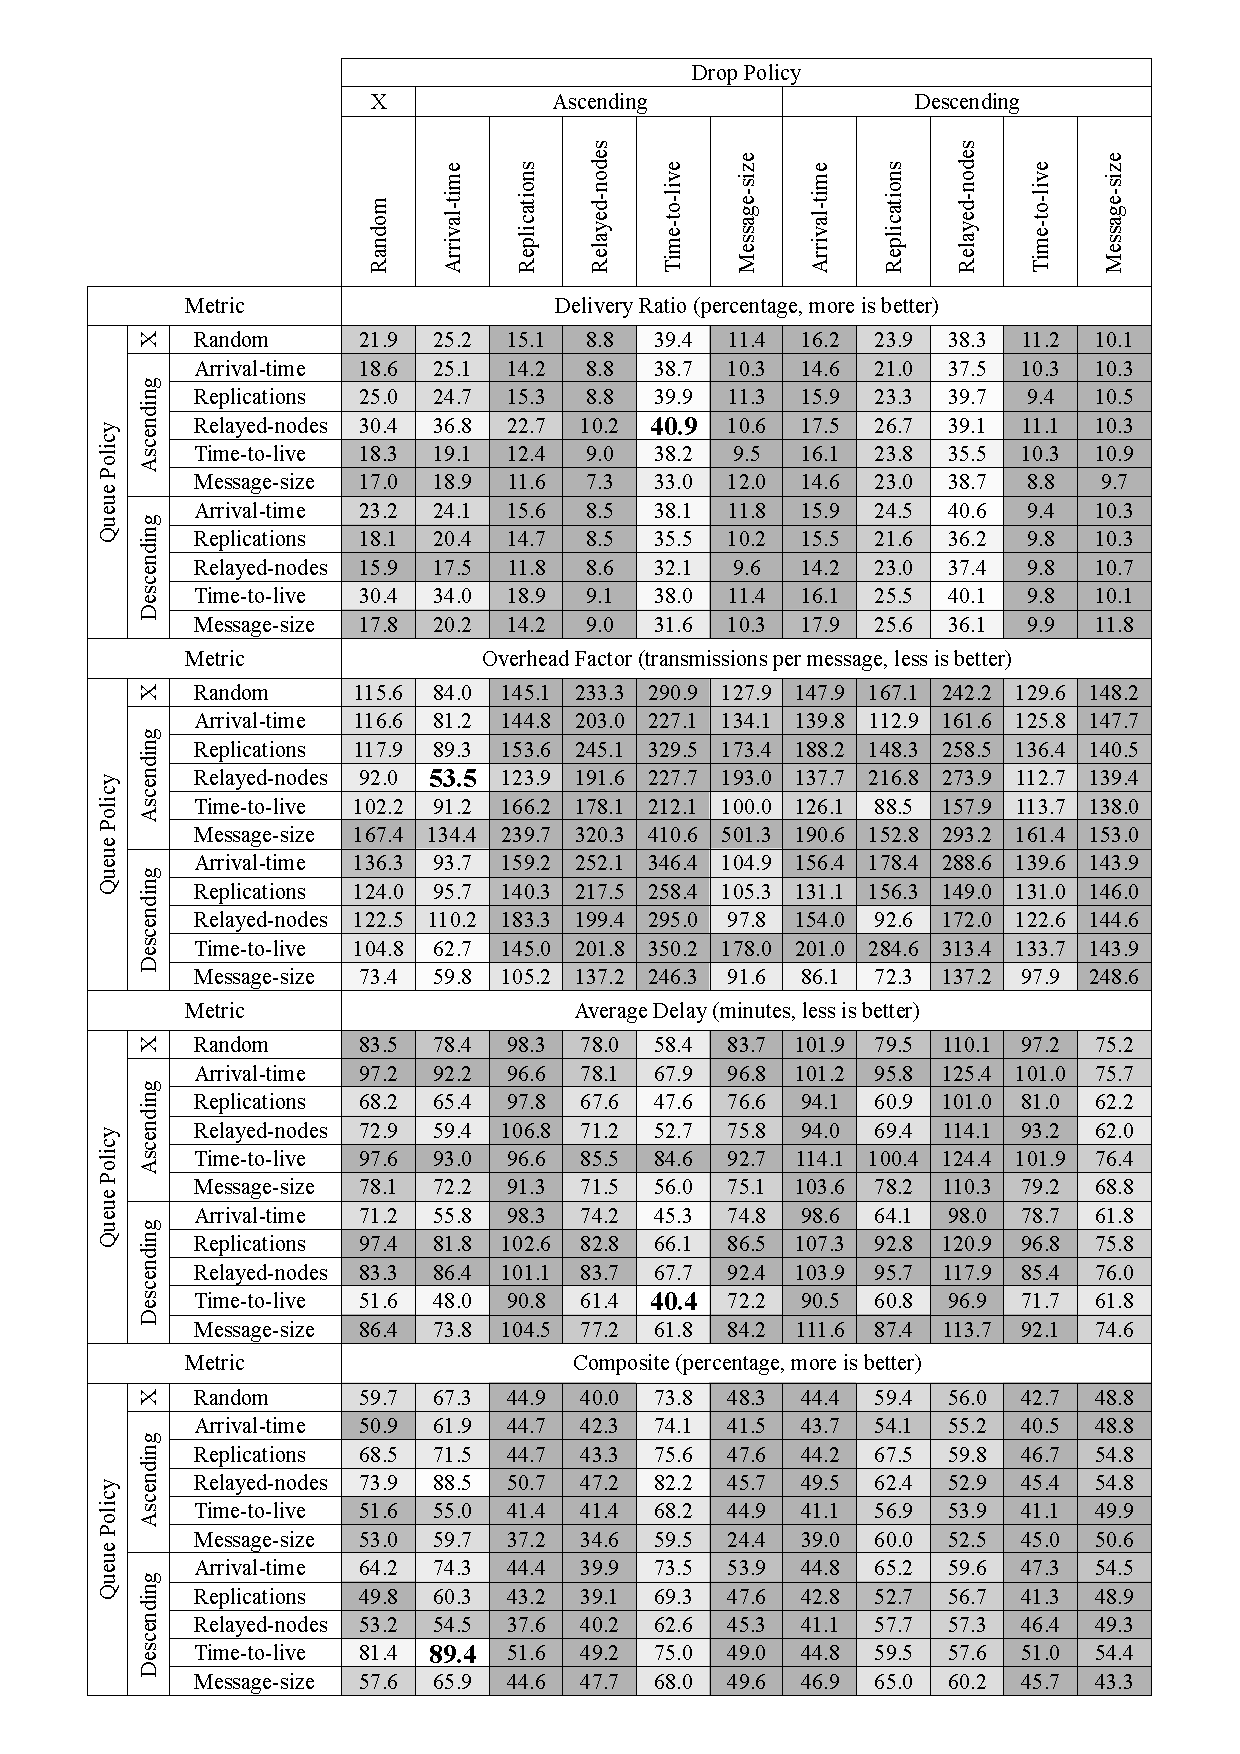
\includegraphics[width=0.95\textwidth]{graphics/tables/scenario1}
	\caption{Scenario 1}
	\label{results:scenario1}
\end{figure*}

\begin{figure*}[h]
	\centering
	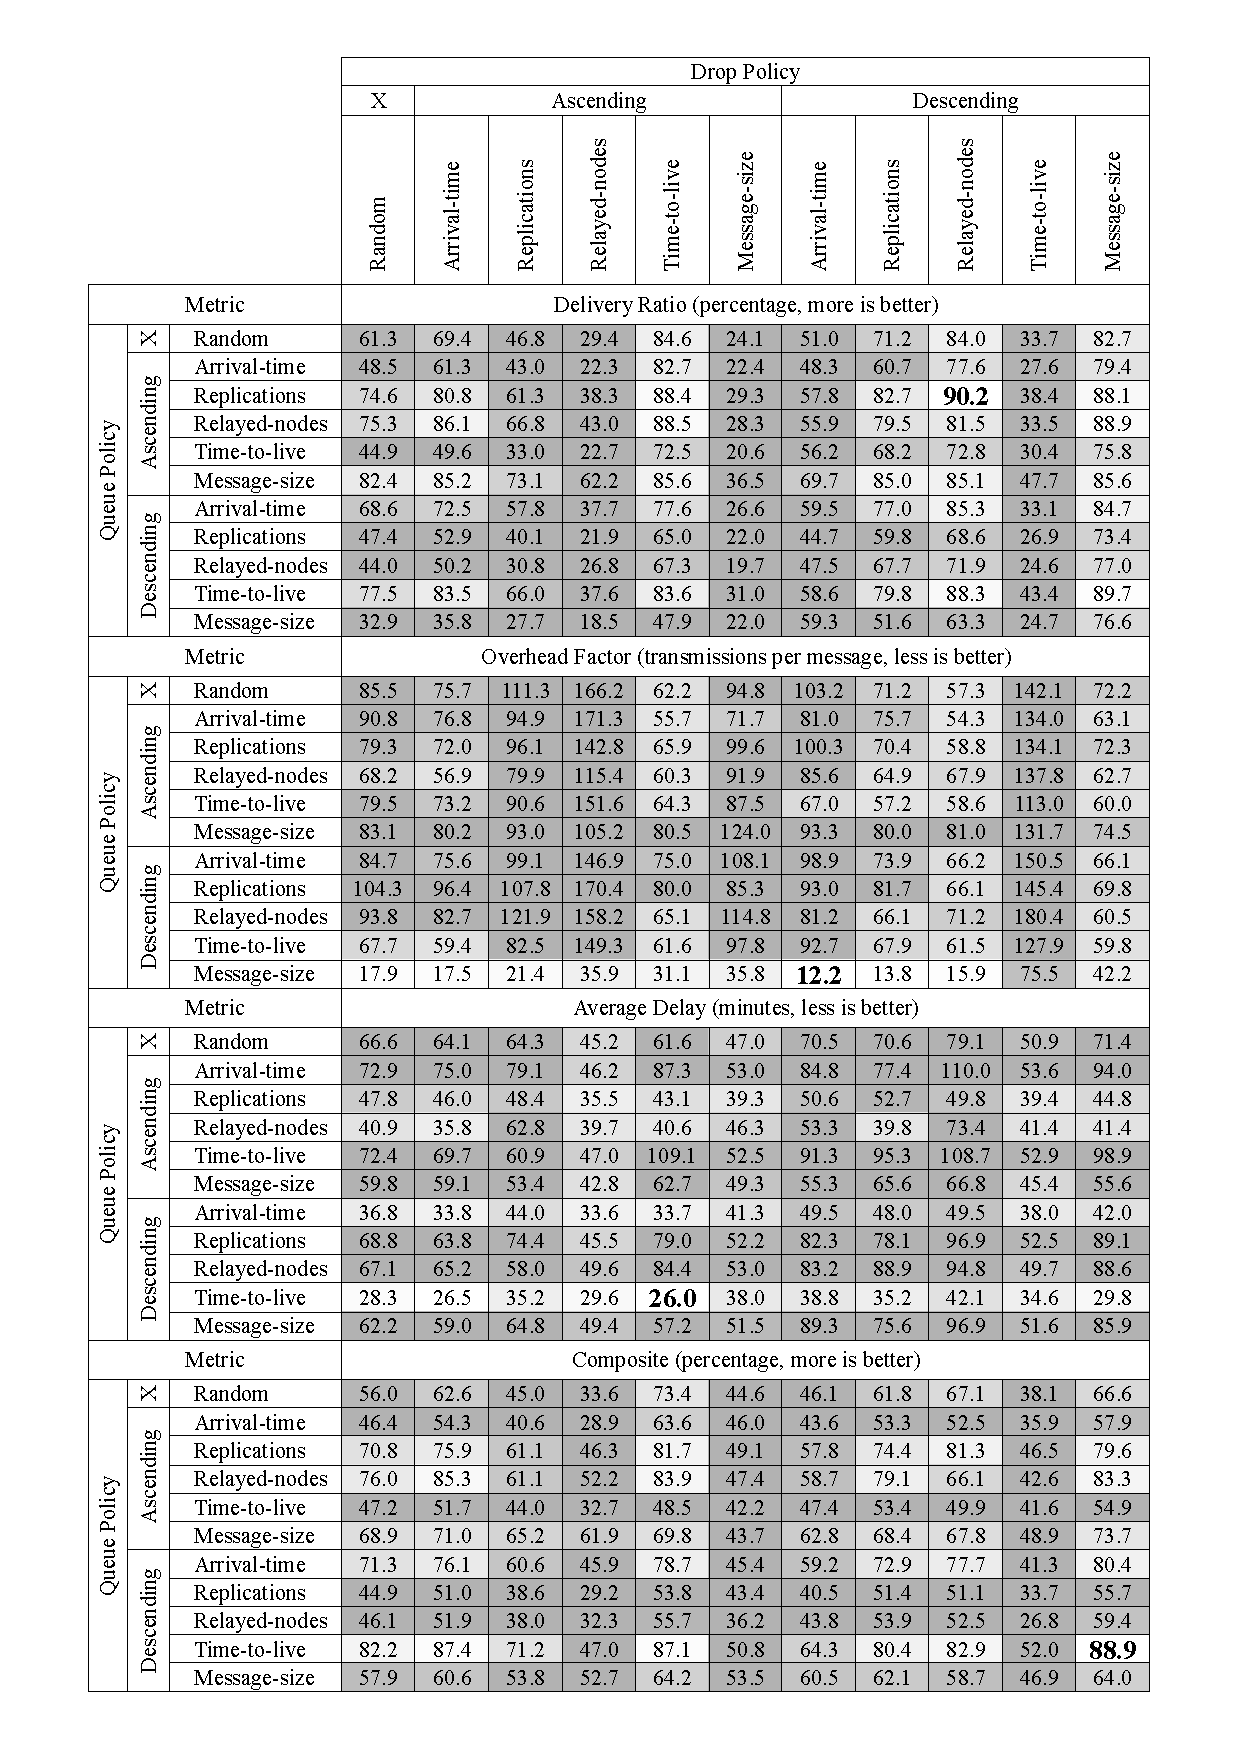
\includegraphics[width=0.95\textwidth]{graphics/tables/scenario2}
	\caption{Scenario 2}
	\label{results:scenario2}
\end{figure*}

\begin{figure*}[h]
	\centering
	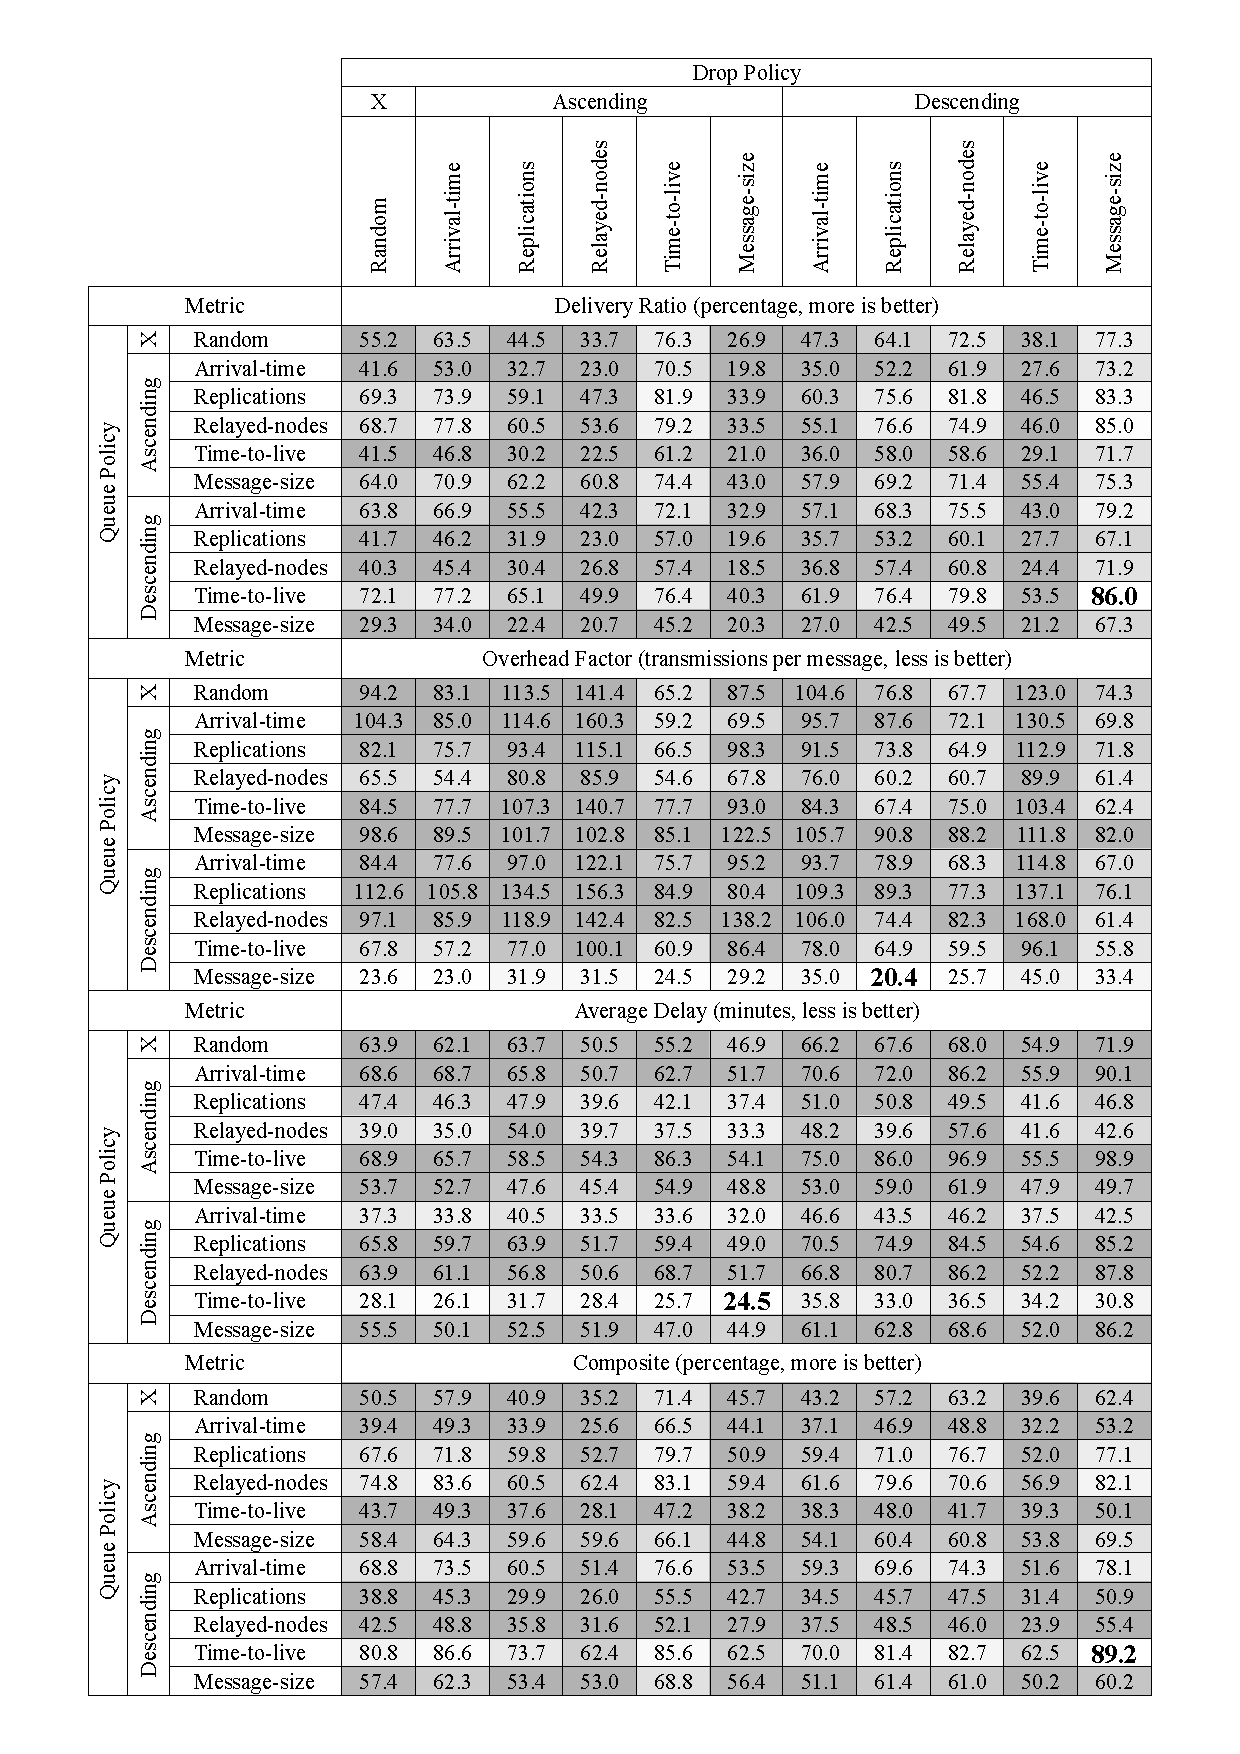
\includegraphics[width=0.95\textwidth]{graphics/tables/scenario3}
	\caption{Scenario 3}
	\label{results:scenario3}
\end{figure*}

\begin{figure*}[h]
	\centering
	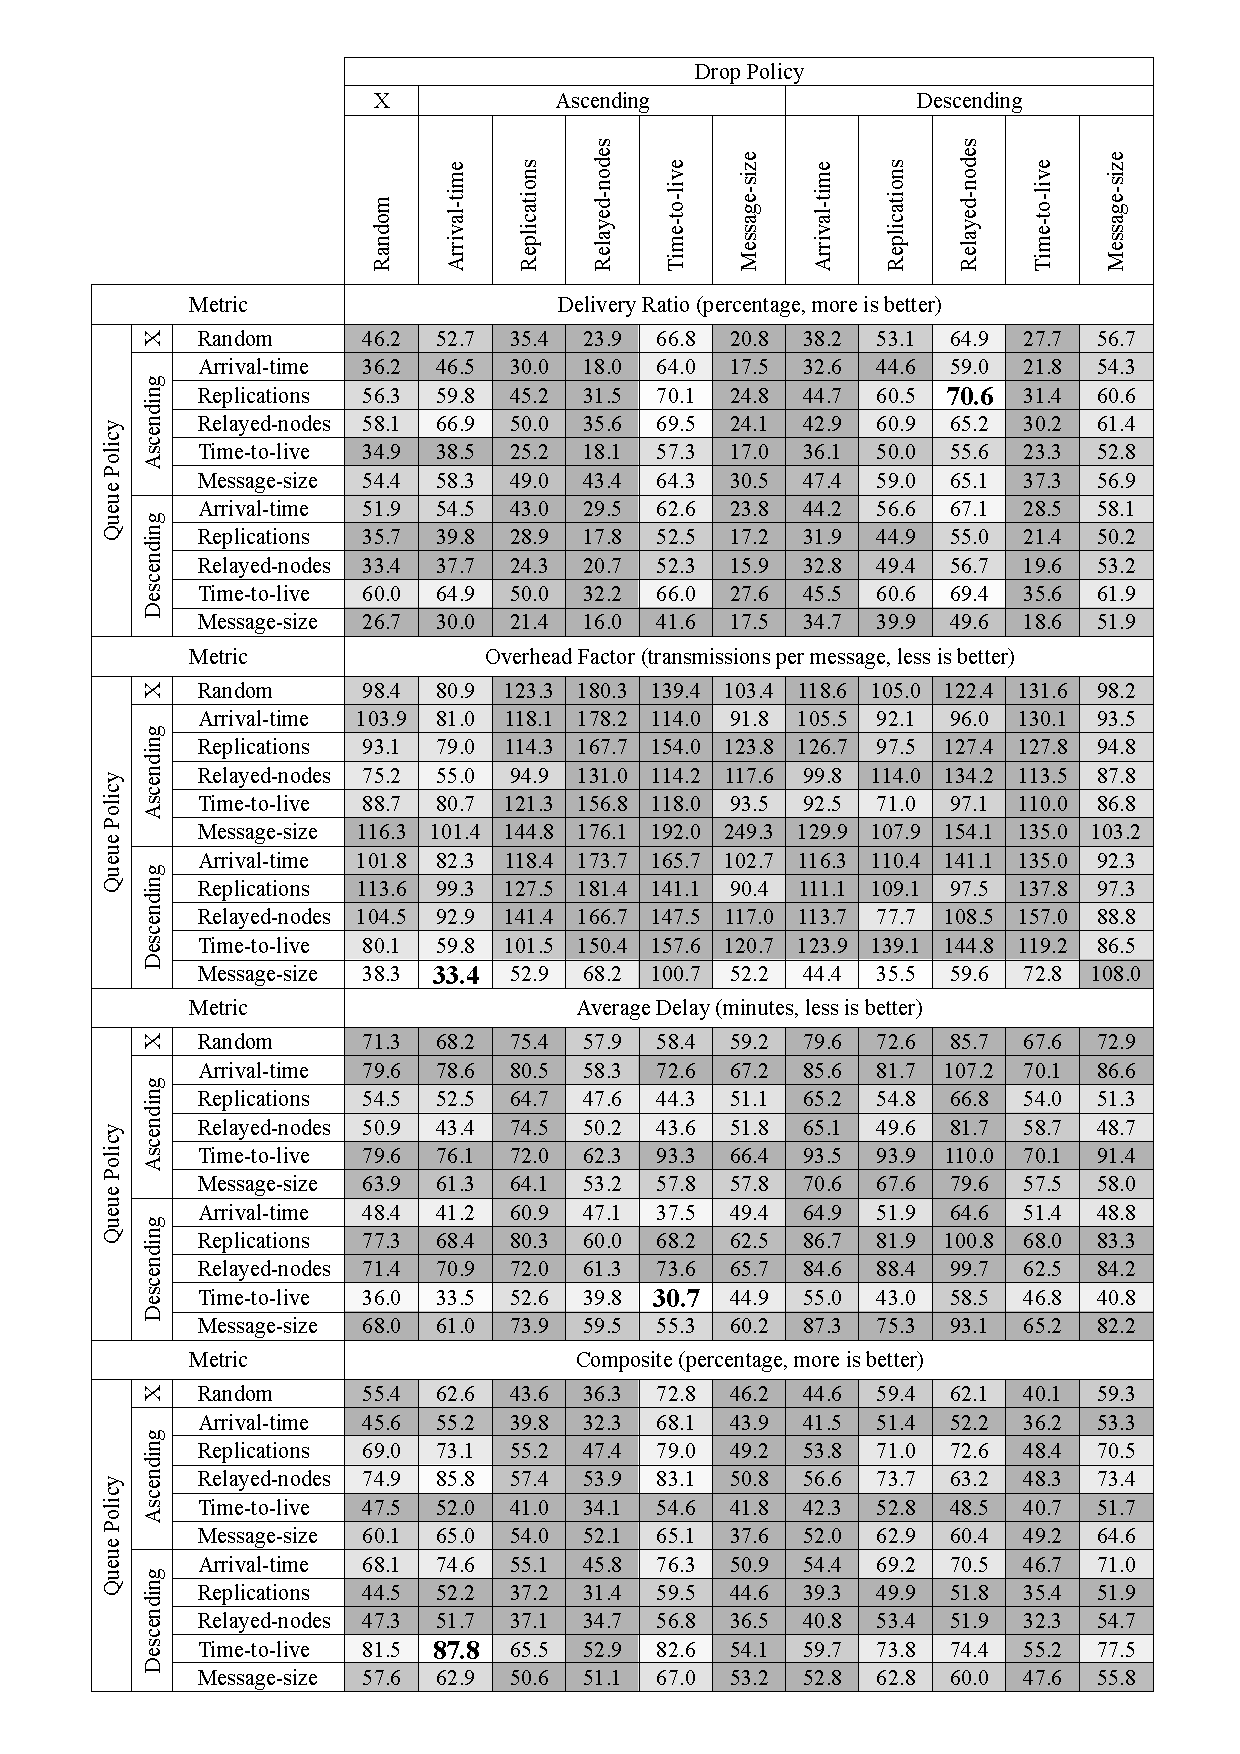
\includegraphics[width=0.95\textwidth]{graphics/tables/composite_scenario_evaluation}
	\caption{Composite Scenario Evaluation}
	\label{results:compositescenario}
\end{figure*}




% \bibliographystyle{IEEEtranKG}
\bibliographystyle{IEEEtran2}
\bibliography{HHU_2015SS_Opp-P2P-Networks___Christopher_Probst___MO3.bib}

\end{document}